%&bericht

%%%%%%%%%%%%%%%%%%%%%%%%%%%%%%%%%%%%%%%%%%%%%%%%%%%%%%%%%%%%%%%%%%%%%%%%%%%%%%%
%% Descr:       Vorlage für Berichte der DHBW-Karlsruhe
%% Author:      Prof. Dr. Jürgen Vollmer, juergen.vollmer@dhbw-karlsruhe.de
%% $Id: bericht.tex,v 1.25 2020/03/13 15:07:45 vollmer Exp $
%%  -*- coding: utf-8 -*-
%%%%%%%%%%%%%%%%%%%%%%%%%%%%%%%%%%%%%%%%%%%%%%%%%%%%%%%%%%%%%%%%%%%%%%%%%%%%%%%

\documentclass[
   ngerman          % neue deutsche Rechtschreibung
  ,a4paper          % Papiergrösse
% ,twoside          % Zweiseitiger Druck (rechts/links)
% ,10pt             % Schriftgrösse
  ,11pt
% ,12pt
  ,pdftex
%  ,disable         % Todo-Markierungen auschalten
]{report}

% Bitte die Codierung Ihrer Dateien auswählen:
% \usepackage[latin1]{inputenc}    % Für UNIX mit ISO-LATIN-codierten Dateien
% \usepackage[applemac]{inputenc}  % Für Apple Mac
% \usepackage[ansinew]{inputenc}   % Für Microsoft Windows
\usepackage[utf8]{inputenc}        % UTF-8 codierte Dateien
                                   % Dieses Dokument ist unter Unix erstellt, daher
                                   % wird diese Input-Codierung benutzt.
\setlength{\marginparwidth}{2cm}
\usepackage{bericht}

%% ACHTUNG, wenn man eine eigene Formatdatei (bericht.fmt) benutzt, werden Änderungen an bericht.sty
%% erst wirksam, wenn die Format-Datei neu erzeugt wurde!!!
%% Genauer alle Änderungen, die textuell vor der nächsten Zeile ".... endofdump...." stehen
%% werden erst wirksam, wenn die Formatdatei neu erzeugt wurde
\csname endofdump\endcsname

%%listing settings
\lstset{showstringspaces=false}

%%%%%%%%%%%%%%%%%%%%%%%%%%%%%%%%%%%%%%%%%%%%%%%%%%%%%%%%%%%%%%%%%%%%%%%%%%%%%%%
%% Angaben zur Arbeit
%%%%%%%%%%%%%%%%%%%%%%%%%%%%%%%%%%%%%%%%%%%%%%%%%%%%%%%%%%%%%%%%%%%%%%%%%%%%%%%

\newcommand{\Autor}{Felix Manuel Gervasi}
\newcommand{\AutorZwei}{Alena Sutiagina}
\newcommand{\MatrikelNummer}{1052491}
\newcommand{\Kursbezeichnung}{TINF20B4}

\newcommand{\FirmenName}{}
\newcommand{\FirmenStadt}{}
\newcommand{\FirmenLogoDeckblatt}{}

% Falls es kein Firmenlogo gibt:
%  \newcommand{\FirmenLogoDeckblatt}{}

\newcommand{\BetreuerFirma}{Prof. Dr. Jörn Eisenbiegler}

%%%%%%%%%%%%%%%%%%%%%%%%%%%%%%%%%%%%%%%%%%%%%%%%%%%%%%%%%%%%%%%%%%%%%%%%%%%%%%%%%%%%%

% Wird auf dem Deckblatt und in der Erklärung benutzt:
\newcommand{\Was}{Studienarbeit}

%%%%%%%%%%%%%%%%%%%%%%%%%%%%%%%%%%%%%%%%%%%%%%%%%%%%%%%%%%%%%%%%%%%%%%%%%%%%%%%%%%%%%

\newcommand{\Titel}{Bedienung einer Getränkemischmaschine über Sprachbefehle}
\newcommand{\AbgabeDatum}{31. März 2023}

\newcommand{\Dauer}{6 Monate}

\newcommand{\Abschluss}{Bachelor of Science}

\newcommand{\Studiengang}{Angewandte Informatik}

\hypersetup{%%
  pdfauthor={\Autor},
  pdftitle={\Titel},
  pdfsubject={\Was}
}

% um die nervigen Errors zu eliminieren, die auftauchen, wenn man versucht
% einen Zeilenumbruch manuell innerhalb eines section-Titels einzufügen
% s. https://tex.stackexchange.com/questions/10555/hyperref-warning-token-not-allowed-in-a-pdf-string
\pdfstringdefDisableCommands{%
  \def\\{}%
}

%%%%%%%%%%%%%%%%%%%%%%%%%%%%%%%%%%%%%%%%%%%%%%%%%%%%%%%%%%%%%%%%%%%%%%%%%%%%%%%

% Wenn \includeonly{..} benutzt wird, werden nur diese Kaptitel ausgegeben.
%\includeonly{
%  abk
% ,kapitel1
% ,kapitel2
% ,changelog
%}

%%%%%%%%%%%%%%%%%%%%%%%%%%%%%%%%%%%%%%%%%%%%%%%%%%%%%%%%%%%%%%%%%%%%%%%%%%%%%%%

% Benutzt man das "biblatex"-Paket, dann muß das hier stehen:
% siehe auch die mit BIBLATEX markierten Zeilen in bericht.sty
\bibliography{bericht}

\graphicspath{{img/}}

\begin{document}

%%%%%%%%%%%%%%%%%%%%%%%%%%%%%%%%%%%%%%%%%%%%%%%%%%%%%%%%%%%%%%%%%%%%%%%%%%%%%%%

\begin{titlepage}
  \begin{center}
    \vspace*{-2cm}
    \FirmenLogoDeckblatt\hfill
\includegraphics[width=4cm]{DHBW_Logo_KA}\\[2cm]
    {\Huge \Titel}\\[1cm]
    {\Huge\scshape \Was}\\[1cm]
    {\large für die Prüfung zum}\\[0.5cm]
    {\Large \Abschluss}\\[0.5cm]
    {\large des Studienganges \Studiengang}\\[0.5cm]
    {\large an der}\\[0.5cm]
    {\large Dualen Hochschule Baden-Württemberg Karlsruhe}\\[0.5cm]
    {\large von}\\[0.5cm]
    {\large\bfseries \Autor}\\[0.5cm]
    {\large und}\\[0.5cm]
    {\large\bfseries \AutorZwei}\\[1cm]
    {\large Abgabedatum \AbgabeDatum}
    \vfill
  \end{center}
  \begin{tabular}{l@{\hspace{2cm}}l}
    Bearbeitungszeitraum          & \Dauer           \\
    Matrikelnummer                & \MatrikelNummer  \\
    Kurs                          & \Kursbezeichnung \\
    Ausbildungsfirma              & \FirmenName      \\
                                  & \FirmenStadt     \\
    Betreuer der Studienarbeit & \BetreuerFirma   \\
  \end{tabular}
\end{titlepage}

%%%%%%%%%%%%%%%%%%%%%%%%%%%%%%%%%%%%%%%%%%%%%%%%%%%%%%%%%%%%%%%%%%%%%%%%%%%%%%%

%%%%%%%%%%%%%%%%%%%%%%%%%%%%%%%%%%%%%%%%%%%%%%%%%%%%%%%%%%%%%%%%%%%%%%%%%%%%%%%
%% Descr:       Vorlage für Berichte der DHBW-Karlsruhe, Erklärung
%% Author:      Prof. Dr. Jürgen Vollmer, vollmer@dhbw-karlsruhe.de
%% $Id: erklaerung.tex,v 1.11 2020/03/13 14:24:42 vollmer Exp $
%% -*- coding: utf-8 -*-
%%%%%%%%%%%%%%%%%%%%%%%%%%%%%%%%%%%%%%%%%%%%%%%%%%%%%%%%%%%%%%%%%%%%%%%%%%%%%%%

% In Bachelorarbeiten muss eine schriftliche Erklärung abgegeben werden.
% Hierin bestätigen die Studierenden, dass die Bachelorarbeit, etc.
% selbständig verfasst und sämtliche Quellen und Hilfsmittel angegeben sind. Diese Erklärung
% bildet das zweite Blatt der Arbeit. Der Text dieser Erklärung muss auf einer separaten Seite
% wie unten angegeben lauten.

\newpage
\thispagestyle{empty}
\begin{framed}
\begin{center}
\Large\bfseries Erklärung
\end{center}
\medskip
\noindent
% siehe §5(3) der \enquote{Studien- und Prüfungsordnung DHBW Technik} vom 29.\,9.\,2017 und Anhang 1.1.13
Ich versichere hiermit, dass ich meine \Was mit dem Thema:
\enquote{\Titel}
selbstständig verfasst und keine anderen als die angegebenen Quellen und Hilfsmittel benutzt habe. Ich versichere zudem, dass die eingereichte elektronische Fassung mit der gedruckten Fassung übereinstimmt.
\vspace{3cm} \\
\underline{\hspace{4cm}}\hfill\underline{\hspace{6cm}}\\
Ort~~~~~Datum\hfill Unterschrift\hspace{4cm}
\end{framed}

%%%%%%%%%%%%%%%%%%%%%%%%%%%%%%%%%%%%%%%%%%%%%%%%%%%%%%%%%%%%%%%%%%%%%%%%%%%%%%%
\endinput
%%%%%%%%%%%%%%%%%%%%%%%%%%%%%%%%%%%%%%%%%%%%%%%%%%%%%%%%%%%%%%%%%%%%%%%%%%%%%%%


%%%%%%%%%%%%%%%%%%%%%%%%%%%%%%%%%%%%%%%%%%%%%%%%%%%%%%%%%%%%%%%%%%%%%%%%%%%%%%%

\begin{abstract}
  TODO
\end{abstract}

\renewcommand{\abstractname}{Abstract}
\begin{abstract}
  TODO
\end{abstract}

\newpage
\pagenumbering{roman}
\newcounter{roman-numbering}
\tableofcontents           % Inhaltsverzeichnis hier ausgeben
\clearpage
\addcontentsline{toc}{chapter}{Abbildungsverzeichnis}
\listoffigures             % Liste der Abbildungen
%\listoftables              % Liste der Tabellen
\clearpage
\addcontentsline{toc}{chapter}{Listingverzeichnis}
\lstlistoflistings         % Liste der Listings
%\listofequations           % Liste der Formeln

% Jetzt kommt der "eigentliche" Text
%%%%%%%%%%%%%%%%%%%%%%%%%%%%%%%%%%%%%%%%%%%%%%%%%%%%%%%%%%%%%%%%%%%%%%%%%%%%%%
%% Descr:       Vorlage für Berichte der DHBW-Karlsruhe, Datei mit Abkürzungen
%% Author:      Prof. Dr. Jürgen Vollmer, vollmer@dhbw-karlsruhe.de
%% $Id: abk.tex,v 1.4 2017/10/06 14:02:03 vollmer Exp $
%% -*- coding: utf-8 -*-
%%%%%%%%%%%%%%%%%%%%%%%%%%%%%%%%%%%%%%%%%%%%%%%%%%%%%%%%%%%%%%%%%%%%%%%%%%%%%%%

\chapter*{Abkürzungsverzeichnis}                   % chapter*{..} -->   keine Nummer, kein "Kapitel"
						         % Nicht ins Inhaltsverzeichnis
\addcontentsline{toc}{chapter}{Akürzungsverzeichnis}   % Damit das doch ins Inhaltsverzeichnis kommt

% Hier werden die Abkürzungen definiert
\begin{acronym}[BIS]
  % \acro{Name}{Darstellung der Abkürzung}{Langform der Abkürzung}
 \acro{Abk}[Abk.]{Abkürzung}

 % Folgendes benutzen, wenn der Plural einer Abk. benöigt wird
 % \newacroplural{Name}{Darstellung der Abkürzung}{Langform der Abkürzung}
 \newacroplural{Abk}[Abk-en]{Abkürzungen}

 \acro{H2O}[\ensuremath{H_2O}]{Di-Hydrogen-Monoxid}

 % Wenn neicht benutzt, erscheint diese Abk. nicht in der Liste
 \acro{NUA}{Not Used Acronym}
 \acro{HTTP}{Hypertext Transfer Protocol}
 \acro{NLP}{Natural Language Processing}
 \acro{AIML}{Artificial Intelligence Markup Language}
 \acro{XML}{eXtensible Markup Language}
 \acro{NLTK}{Natural Language Toolkit}
 \acro{TF}{Term Frequency}
 \acro{IDF}{Inverse Document Frequency}
 \acro{RBM}{Restricted Boltzmann Machines}
 \acro{GAN}{Generative Adversarial Network}
 \acro{RNN}{Recurrent Neural Networks}
 \acro{IoT}{Internet der Dinge}
 \acro{KI}{Künstlichen Intelligenz}
 \acro{ML}{Machine Learning}
 \acro{UI}{User Interface}
 \acro{RAM}{Read Only Memory}
 \acro{CFG}{Context-free grammar}
 \acro{NLTK}{Natural Language Toolkit}
 \acro{API}{Application Programming Interface}
 \acro{CMU}{Carnegie Mellon University}
 \acro{BOW}{Bag Of Words}
 \acro{seq2seq}{sequence-to-sequence}
 \acro{GB}{Gigabyte}
 \acro{TF-IDF}{Term Frequency-Inverse Document Frequency}
 \acro{MLP}{Multilayer Perceptron}
 \acro{LSA}{Latent Semantic Analysis}
 \acro{SWZ}{Singulärwertzerlegung}
 \acro{SVD}{Singular Value Decomposition}
 \acro{MLP}{Mehrschichtiges Perzeptron}
\end{acronym}

              % Abkürzungsverzeichnis
\setcounter{roman-numbering}{\value{page}}
\pagenumbering{arabic}
\chapter{Einleitung}
% Einführung: Interesse vom Leser wecken
Die Informationstechnik versteckt sich heutzutage fast überall - selbst dort, wo sie von den meisten Menschen nicht vermutet werden würde. Beispiele hierfür sind Autos, Kaffeemaschinen, Zahnbürsten, Rasierer, Küchengeräte und vieles mehr. Grund dafür ist die fortschreitende Möglichkeit der Miniaturisierung von Computern, sodass diese nahezu überall verbaut werden können. Beispielsweise können Mikrochips in der Kaffeemaschine dafür sorgen, dass die richtige Menge an Kaffee serviert wird oder der Füllstand der einzelnen Behälter angezeigt werden kann. Solche Systeme, die Informationen mit Hilfe eines Computers verarbeiten und dabei mit ihrer Umgebung derartig \glqq{}verschmelzen\grqq{}, nennt man auch \textit{embedded systems} (z. Dt. \textit{eingebettete Systeme}) \cite{marwedel_eingebettete_2021}.\\\\
Der aktuelle Trend des \ac{IoT} führt zu einem noch größeren Anstieg eingebetteter Systeme im Alltag. Im \ac{IoT} geht es speziell um eingebettete Systeme, die internetfähig (vernetzt) sind. Nach Schätzungen des Marktforschungsunternehmens \textit{Gartner} gab es im Jahr 2017 8,4 Milliarden solcher vernetzten Geräte weltweit \cite{jansen_digitalisierung_2017}. Das die Menge der vernetzten Geräte als Teilmenge der eingebetteten Systeme betrachtet werden kann ist damit zu rechnen, dass deren Anzahl sogar weit größer ausfällt.

\section{Aufgabenstellung}
Im Rahmen dieser Arbeit geht es um die Sprachsteuerung einer Getränkemischmaschine, die in diesem Fall als eingebettetes System zu verstehen ist und in einer vorangegangenen Arbeit bereits konzipiert und gebaut wurde. Sie verfügt derzeit über ein Touch-Display zur Bedienung durch den Benutzer. Ziel der Arbeit ist es zusätzlich eine natürlichsprachliche Interaktion mit der Maschine zu ermöglichen, die mindestens den Funktionsumfang besitzt, der aktuell über die Bildschirmeingabe möglich ist. Dabei soll die Maschine nicht nur in der Lage sein die natrüliche Sprache des Benutzers in ein geeignetes Format umzuwandeln, sodass die Maschine den korrekten Befehl ausführt. Sie soll auch in der Lage sein dem Benutzer zu Antworten, sodass die Illusion einer Konversation mit der Maschine entsteht.

\section{Vorgehen}
Zunächst müssen die Sprachverarbeitung und Spracherkennung betrachtet werden. Die Sprachverarbeitung dient der Interpretation des Gesprochenen um eine geeignete Antwort auszugeben und dem Übersetzen in einen Maschinenbefehl. Im Rahmen dieser Arbeit sollen dafür Verfahren und Techniken der \ac{KI} und des \ac{ML} eingesetzt werden. Die Spracherkennung beschäftigt sich mit der Aufnahme des Tonsignals bzw. der Schallwellen (bspw. über ein Mikrofon) und dem Umwandeln dieser Signale in Text, sodass dieser an das \ac{KI}-Modell weitergereicht werden kann.\\\\
Bei der Arbeit mit eingebetteten Systemen muss man sich der vorhandenen Hardwareleistung und den benötigten Hardwareanforderungen bewusst sein, da diese meist sehr begrenzt ist. Deshalb werden im Rahmen dieser Arbeit verschiedene Ansätze diskutiert, wie und wo die einzelnen Schritte und Berechnungen ablaufen sollen (s. Kapitel \ref{chap:konzept}).
\endinput
\chapter{Stand der Technik}
\section{Getränkemischmaschine}
\section{Hardware}
\section{Sprachverarbeitung}
Im Zuge des technologischen Fortschritts nutzen die Menschen heutzutage zunehmend Sprachassistenten für verschiedene Aufgaben. 
Einer der Hauptvorteile der Sprachsteuerung ist die Bequemlichkeit und Geschwindigkeit, mit der Aufgaben erledigt werden können, ohne dass man tippen oder mit der Maus klicken muss. 
Sprachassistenten nutzen die Verarbeitung natürlicher Sprache, um Befehle zu erkennen und zu verstehen, die der Nutzer laut ausspricht.\\\\
Die Verarbeitung natürlicher Sprache - \ac{NLP} - ist eine wichtige Technologie, die es Computern ermöglicht, die von Menschen verwendete natürliche Sprache zu verstehen. 
Diese Technologie ermöglicht es Computern, menschliche Sprache zu erkennen und zu interpretieren und Text und Sprache in natürlicher Sprache zu erzeugen. 
Im Bereich der Sprachsteuerung spielt \ac{NLP} eine Schlüsselrolle bei der Erkennung von Sprache und dem Verstehen von Befehlen, die der Benutzer laut ausspricht. 
Es wird verwendet, um die Sprache des Benutzers in Text umzuwandeln, den ein Computer verstehen und verarbeiten kann.
Um dies zu erreichen, verwendet \ac{NLP} eine Vielzahl von Techniken und Technologien, darunter maschinelles Lernen, Tonanalyse, syntaktische Analyse und mehr. \cite{jurafsky_speech_2009}\\\\
Im Rahmen dieses Projekts erfordert die Implementierung der Sprachsteuerung einer Getränkemischmaschine die Verarbeitung natürlicher Sprache, damit die Maschine Befehle verstehen kann, die der Benutzer laut ausspricht. 
Dieses Projekt ähnelt einem Chatbot, bei dem der Benutzer eine Frage stellen oder einen Befehl geben kann und der Chatbot führt die entsprechende Aktion aus. 
Die Verarbeitung natürlicher Sprache ist für die Entwicklung eines solchen Sprachsteuerungssystems unerlässlich und ermöglicht es der Maschine, Befehle in natürlicher Sprache zu verstehen und auszuführen.\\\\
Eine der wichtigsten Komponenten der Verarbeitung natürlicher Sprache ist die Spracherkennung und das Syntaxanalyseverfahren. 
Bei der Spracherkennung kommen Deep-Learning-Techniken zum Einsatz, die es einem Computer ermöglichen, Sprachlaute zu erkennen und in Text zu übersetzen. 
Anschließend wird das Syntaxanalyseverfahren verwendet, um die Satzstruktur zu bestimmen und Schlüsselwörter und -sätze hervorzuheben, die zur Bestimmung des Benutzerbefehls verwendet werden können.
Auch die Tonwertanalyse ist ein wichtiger Bestandteil der Verarbeitung natürlicher Sprache. 
Mit Hilfe der Tonalitätsanalyse lässt sich die emotionale Färbung des Textes bestimmen, was für die Ermittlung der Absicht des Nutzers nützlich sein kann. 
Da die Tonwertanalyse im Rahmen dieser Arbeit nicht relevant ist, wird sie nicht weiter erörtert.\\\\
Darüber hinaus werden grammatik- und regelbasierte Technologien zur Verarbeitung natürlicher Sprache eingesetzt. 
Diese Technologien werden eingesetzt, um die korrekte Struktur des Benutzerbefehls zu bestimmen und Schlüsselwörter hervorzuheben, die zur Durchführung von Aktionen verwendet werden können. 
Außerdem werden Techniken des maschinellen Lernens eingesetzt, damit der Computer aus früheren Befehlen und Aktionen \glqq{}lernen\grqq{} kann, was die Genauigkeit der Erkennung von Benutzerbefehlen verbessert.\\\\
Daher ist der Einsatz von Technologien zur Verarbeitung natürlicher Sprache für das Projekt der Sprachmischmaschine unerlässlich. 
Die Verarbeitung natürlicher Sprache wird es der Maschine ermöglichen, die Befehle zu verstehen und zu verarbeiten, die der Benutzer laut ausspricht und die entsprechenden Aktionen durchzuführen.
\subsection{Verarbeitung natürlicher Sprache}
\subsection{Tokenisierung von Wörtern}
\subsection{Vektoren von Wörtern}
\subsection{Syntaktische Analyse}
\subsection{Ansätze für die Erstellung eines Chatbots}\label{sec:ansaetze_erstellung_chatbots}
Derzeit gibt es vier Hauptansätze für die Erstellung eines Chatbots \cite{lane_natural_2019}:
\begin{itemize}
    \item Musterabgleich: Musterabgleich und Antwortvorlagen (vorgefertigte Antworten)
    \item Grounding: logische Wissensgraphen und das Ziehen von Schlussfolgerungen aus diesen basierend auf diesen Graphen
    \item Suche: Abrufen von Text
    \item Generierungsmethoden: Statistik und maschinelles Lernen
\end{itemize}
Die vier grundlegenden Ansätze zur Erstellung von Chatbots lassen sich kombinieren, was zu benutzerfreundlicheren Chatbots führt. 
Eine Vielzahl von Anwendungen nutzen alle vier grundlegenden Methoden. 
Hybride Chatbots unterscheiden sich hauptsächlich darin, wie genau sie diese Ansätze kombinieren und wie viel Gewicht auf jeden einzelnen Ansatz gelegt wird.
\subsubsection{Musterabgleich}
Bei den ersten Chatbots basierte die Antwort auf die Nachricht eines Benutzers auf einem Mustervergleich. 
Diese Chatbots suchen nach Mustern im eingehenden Text und geben eine feste (gemusterte) Antwort, wenn eine Übereinstimmung gefunden wird \cite{woudenberg_chatbot_2014}.\\\\
Solche rudimentären Dialogsysteme sind vor allem in automatisierten Benutzerunterstützungssystemen mit interaktiven Sprachmenüs nützlich, wo es möglich ist, das Gespräch an einen Menschen weiterzuleiten, wenn der Chatbot keine Antwortmuster mehr hat.\\\\
Da es viele \ac{NLP}-Dienstprogramme in Python-Paketen gibt, ist es möglich, komplexere Chatbots auf der Grundlage von Mustervergleichen zu erstellen, indem man die Bot-Logik nach und nach direkt in Python mit regulären Ausdrücken und Suchmustern aufbaut.\\\\
1995 machte sich Richard Wallace daran, einen allgemeinen Rahmen für die Erstellung von Chatbots auf der Grundlage des Pattern-Matching-Ansatzes zu schaffen. Zwischen 1995 und 2002 schuf seine Entwicklergemeinschaft die \ac{AIML} zur Beschreibung von Mustern und Chatbot-Antworten.\\\\
\ac{AIML} ist eine deklarative Sprache, die auf dem \ac{XML}-Standard basiert, der die Sprachkonstrukte und Datenstrukturen einschränkt, die im Bot verwendet werden dürfen. \cite{noauthor_aiml_nodate}
Ein Chatbot, der auf \ac{AIML} basiert, sieht folgendermaßen aus:
\begin{figure}[H]
    \centering
    \fbox{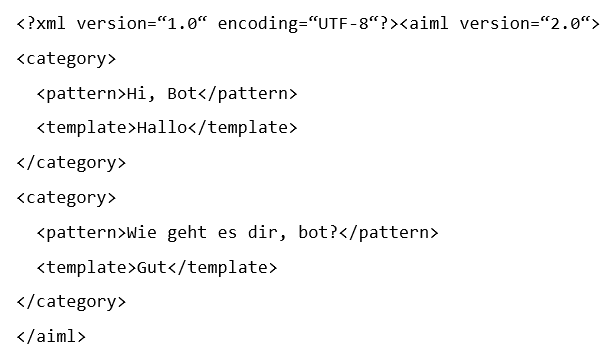
\includegraphics[width=0.8\textwidth]{Bilder_Kapitel_2/aiml_bot.png}}
    \caption{\label{figure:Aiml_Bot}\ac{AIML} Chatbot}
\end{figure}
\noindent
Eine der Einschränkungen von \ac{AIML} ist die Art der Muster, die abgeglichen werden können und auf die reagiert wird. 
Der \ac{AIML}-Kern (Pattern Matching Engine) reagiert nur auf Eingabetext, der einem vom Entwickler manuell vorgegebenen Muster entspricht. 
Unscharfe Suchanfragen, Smileys, Satzzeichen, Tippfehler oder falsch geschriebene Wörter sind nicht erlaubt, es findet kein automatischer Abgleich statt. 
In \ac{AIML} müssen alle Synonyme manuell einzeln beschrieben werden.
\subsubsection{Grounding}
Die Grounding-Methode ist ein Ansatz zur Erstellung eines Chatbots auf der Grundlage logischer Wissensgraphen und der Durchführung von Schlussfolgerungen auf der Grundlage dieser Graphen. \cite{diana_conversational_2011}
Sie wird verwendet, um natürliche Sprache zu verarbeiten und sie dem Verständnis des Bots zuzuordnen. Das Wesentliche an der Grounding-Methode ist, dass der Chatbot nicht nur die Textnachrichten, sondern auch den Kontext und die Umgebung verarbeitet, um Anfragen besser zu verstehen und zu beantworten. 
Durch die Extraktion von Informationen wird ein Netz von Verbindungen oder Fakten geschaffen. Dieses Netz logischer Verbindungen zwischen Entitäten - ein Graph oder eine Wissensbasis - kann die Grundlage für die Antworten des Chatbots bilden.\\\\
Ein Beispiel für eine Grounding-Methode ist die Verwendung eines Wissensgraphen zur Beschreibung der Umgebung. 
Ein Wissensgraph enthält Informationen über die Objekte, mit denen der Bot interagieren kann und die Beziehungen zwischen ihnen. 
Ein Wissensgraph könnte zum Beispiel Informationen über ein Glas auf einem Tisch und das darin befindliche Wasser enthalten. 
Wenn ein Benutzer eine Frage stellt, verwendet der Chatbot den Wissensgraphen, um den Kontext der Anfrage zu verstehen und die am besten geeignete Antwort abzuleiten. 
Wenn ein Benutzer zum Beispiel fragt: \glqq{}Wie hoch ist die Temperatur des Wassers in dem Glas auf dem Tisch?\grqq{}, kann der Chatbot Informationen aus dem Wissensgraphen verwenden, um die Frage zu beantworten.\\\\
Ein solcher Wissensgraph kann abgeleitet werden, um Fragen über die in dieser Wissensbasis enthaltene Welt zu beantworten und anschließend können auf der Grundlage der logischen Antworten die Werte der in den Antworten enthaltenen Template-Variablen ausgefüllt werden, um natürlichsprachliche Antworten zu erstellen. 
Ursprünglich wurden auf diese Weise Systeme zur Beantwortung von Fragen eingerichtet, wie z. B. der Watson-Bot von IBM (heutzutage wird für ähnliche Systeme jedoch die Informationssuchemethode verwendet). 
Der Wissensgraph stellt eine Art \glqq{}Erdung\grqq{} des Chatbots in der realen Welt dar.\\\\
Die Erstellung von Chatbots auf der Grundlage von \glqq{}Grounding\grqq{} eignet sich hervorragend für Chatbots, die Fragen generieren, bei denen das zur Beantwortung einer Frage erforderliche Wissen in einer umfangreichen Wissensbasis enthalten ist, die aus einer offenen Datenbank (z. B. Wikidata, Open Mind Common Sense oder DBpedia) bezogen werden kann.\\\\
Einer der Hauptvorteile der Grounding-Methode besteht darin, dass sie sich an ein sich veränderndes Umfeld anpassen kann. 
Wenn der Benutzer zum Beispiel ein Glas Wasser von einem Tisch auf einen anderen stellt, wird der Wissensgraph automatisch aktualisiert, um diese Änderung widerzuspiegeln.\\\\
Die Grounding-Methode hat jedoch auch ihre Grenzen. 
So kann es vorkommen, dass bei der Verarbeitung großer Informationsmengen Zusammenhänge nicht berücksichtigt werden und dem Bot möglicherweise verborgen bleiben.\\\\
Insgesamt ist die Grounding-Methode ein effektiver Ansatz zur Erstellung wissensbasierter Chatbots. 
Sie ermöglicht es dem Bot, Benutzeranfragen besser zu verstehen und eine genauere Antwort zu geben.
\subsubsection{Suche}
Die Informationssuchemethode ist eine der Methoden zum Aufbau von Chatbots, die auf der Extraktion von Informationen aus einer großen Menge von Textinformationen basiert. 
Die Hauptidee der Informationssuchemethode ist die Analyse des Eingabetextes (Benutzeranfrage), die Auswahl von Schlüsselwörtern und Phrasen daraus und die anschließende Suche nach den relevantesten Informationen in der Wissensdatenbank oder in offenen Quellen. \cite{diana_conversational_2011}\\\\
Die Wissensbasis kann auch eine Art \glqq{}Gesprächsprotokoll\grqq{} sein, in Form von Aussage-Antwort-Paaren. 
Dabei sucht der Bot nach früheren Aussagen in den Protokollen früherer Unterhaltungen. 
Der Bot kann nicht nur in den Protokollen seiner eigenen Gespräche suchen, sondern auch in beliebigen Transkripten von Gesprächen zwischen Menschen, Gesprächen zwischen Menschen und Bots oder sogar Gesprächen zwischen Bots.
Aber wie immer gilt: je besser die Eingabedaten, desto besser das Ergebnis. 
Daher ist es notwendig, die Datenbank früherer Gespräche sorgfältig zu säubern und zu organisieren, damit der Bot nach einem qualitativ hochwertigen Gespräch sucht und es dann imitiert.\\\\
Für die Umsetzung der Informationssuchemethode werden verschiedene Algorithmen und Techniken verwendet, z. B. Indizierung und Schlagwortsuche, Kontextsuche, Textanalyse mit Hilfe von maschinellen Lernverfahren usw. 
Die Informationssuchemethode kann in Python mit verschiedenen Bibliotheken und Tools wie \ac{NLTK}, Scikit-learn und Gensim implementiert werden.\\\\
Einer der ersten Schritte bei der Implementierung einer Informationssuchemethode in Python ist die Vorbereitung der Daten. 
Dies erfordert Tokenisierung, Lemmatisierung und die Entfernung von Stopp-Wörtern. 
Als nächstes muss ein Index auf der Grundlage von Schlüsselwörtern erstellt werden. 
Der Index kann auf der Grundlage von Bag-of-Words oder \ac{TF} und \ac{IDF} (TF-IDF-Modelle) erstellt werden. 
Sobald der Index erstellt ist, kann eine Stichwortsuche durchgeführt werden. 
Dazu muss die Benutzeranfrage in einen Vektor umgewandelt und mit den Dokumentvektoren im Index verglichen werden. 
Dies kann mit Hilfe der Scikit-learn-Bibliothek erfolgen \cite{scikit-learn}.
Sobald die relevantesten Dokumente gefunden wurden, können sie in eine Rangfolge gebracht und als Antwort auf die Benutzeranfrage angezeigt werden.\\\\
Der Vorteil der Informationssuchemethode besteht darin, dass sie ein schnelles und genaues Auffinden der gewünschten Informationen ermöglicht, insbesondere wenn die Wissensbasis gut strukturiert ist und genügend Informationen enthält. 
Ein Nachteil dieser Methode ist jedoch, dass sie den Kontext der Anfrage nicht berücksichtigt und nicht immer eine vollständige und genaue Antwort auf die Frage des Nutzers liefert. 
Wenn die Aussage semantisch mit der vom Bot zu beantwortenden übereinstimmt, ist es möglich, die Antwort wortwörtlich und ohne Änderungen wiederzuverwenden. 
Aber selbst wenn die Datenbank alle möglichen Benutzeräußerungen enthält, wird der Bot die Persönlichkeiten der Personen widerspiegeln, die diese Äußerungen machen. 
Wenn die Antworten konsistent sind und von einer Vielzahl von Personen stammen, ist das gut. 
Problematisch wird es jedoch, wenn die Äußerung, auf die der Bot reagieren soll, vom Gesamtkontext des jeweiligen Gesprächs oder von den Umständen in der Umgebung abhängt, die sich seit der Erstellung des Dialogkorpus geändert haben können.\\\\
Beispielsweise sollte der Bot auf die Frage \glqq{}Wie spät ist es?\grqq{} nicht die von der Person gegebene Antwort, sondern die am besten geeignete Aussage aus der Datenbank verwenden. 
Diese Antwort funktioniert nur, wenn die Zeit, zu der die Frage gestellt wurde, mit der Zeit übereinstimmt, zu der die passende Äußerung aus der Datenbank aufgezeichnet wurde. 
Neben dem natürlichsprachlichen Text der Äußerung müssen auch ähnliche Informationen über die Zeit - der Kontext (Zustand) - erfasst und verglichen werden. 
Sie spielt vor allem dann eine wichtige Rolle, wenn die Semantik der Äußerung auf eine aktive Veränderung des im Kontext (Wissensbasis des Chatbots) erfassten Zustands hinweist.\\\\
Um den Zustand (Kontext) in einem Chatbot auf der Grundlage der Informationssuche zu berücksichtigen, kann etwas Ähnliches für einen Chatbot mit Musterabgleich durchgeführt werden, da die Auflistung einer Liste von Benutzeraussagen nur eine andere Art ist, ein Muster zu beschreiben. 
Dies auch ist der Ansatz von Amazon Lex \cite{amazon_lex} und Google Dialogflow \cite{dialogflow_chawla}. 
Anstatt ein starres Muster zu beschreiben, um den Befehl des Benutzers zu erfassen, können der Dialogflow-Engine einfach ein paar Beispiele geliefert werden. 
So wie jedes Muster im Chatbot auf der Grundlage der Musterzuordnung einem Zustand zugeordnet wurde, muss auch hier nur die Aussage-Antwort-Beispielpaare mit dem genannten Zustand verknüpft werden.\\\\
Der suchbasierte Chatbot indiziert also den Korpus der Dialoge, so dass er leicht frühere Aussagen finden kann, die derjenigen ähnlich sind, auf die er antworten muss und antwortet dann mit einer der passenden Aussagen aus dem Korpus, die er sich \glqq{}gemerkt\grqq{} und für eine schnelle Suche indiziert hat. 
Im Allgemeinen ist die Methode der Informationssuche eine der gängigsten und beliebtesten Methoden zum Aufbau von Chatbots, die in verschiedenen Bereichen wie Wirtschaft, Medizin, Tourismus und vielen anderen eingesetzt werden.
\subsubsection{Generierungsmethoden}
Generierungsmethoden sind einer der wichtigsten Ansätze bei der Entwicklung von Chatbots auf der Grundlage künstlicher Intelligenz. 
Sie ermöglichen es Chatbots, Textantworten auf der Grundlage der Analyse der eingehenden Nachricht und des Kontextes des Dialogs zu generieren. 
Die folgenden Generierungsmodelle sind nützlich, um einen kreativen Chatbot zu erstellen, der Dinge sagen kann, die noch niemand zuvor gesagt hat:
\begin{itemize}
    \item Sequenz-zu-Sequenz-Konvertierungsmodelle: Modelle, die darauf trainiert sind, Antworten auf der Grundlage von Eingabesequenzen zu generieren;
    \item \ac{RBM}: Markov-Ketten, die so trainiert werden, dass sie die \glqq{}Energie\grqq{}-Funktion minimieren \cite{chatbot_development_sharma};
    \item \ac{GAN}: statistische Modelle, die darauf trainiert sind, einen Experten, der die Qualität eines Gesprächs bewertet, zu täuschen. \cite{li_adversarial_2017}
\end{itemize}
Die Vorteile des Einsatzes der Generierungsmethoden:
\begin{itemize}
    \item Flexibilität: Generative Methoden können für eine breite Palette von Aufgaben eingesetzt werden, einschließlich Texterstellung, Sprachübersetzung, Verarbeitung natürlicher Sprache und mehr.
    \item Automatisierung: Generative Methoden können auf großen Datensätzen trainiert werden, wodurch die Erstellung von Inhalten automatisiert werden kann.
    \item Qualität: Generative Methoden zeigen eine hohe Qualität bei der Textgenerierung, Sprachübersetzung und anderen Aufgaben der natürlichen Sprachverarbeitung, wenn sie auf einem ausreichend großen Datensatz trainiert werden.
    \item Schnelligkeit: Generative Methoden können schneller arbeiten als Menschen, was die Erstellung von Inhalten mit großer Geschwindigkeit ermöglicht.
\end{itemize}
Die Nachteile der generativen Methoden:
\begin{itemize}
    \item Große Datenmengen für das Training: Generative Methoden benötigen große Datenmengen für das Training, was bei einigen Aufgaben schwierig sein kann, insbesondere wenn nur ein kleiner Datensatz zur Verfügung steht.
    \item Sicherheitsrisiken: Generative Methoden können Inhalte erzeugen, die möglicherweise falsch, unvollständig oder irreführend sind. Dies kann zu Sicherheitsrisiken führen, wenn der generierte Inhalt für wichtige Entscheidungen verwendet wird.
    \item Unterstützungsbedarf: Generative Methoden können erhebliche Unterstützung benötigen, um effektiv zu sein. Dies kann die Modellabstimmung, die Auswahl optimaler Parameter und die Optimierung der Modellleistung auf einer bestimmten Hardwarekonfiguration umfassen.
    \item Modellbeschränkungen: Generative Methoden können Beschränkungen hinsichtlich der Arten von Inhalten haben, die sie erzeugen können, insbesondere wenn sie nur auf bestimmte Datentypen trainiert wurden.
\end{itemize}
Eine der beliebtesten Methoden zur Texterstellung ist die sequence-to-sequence-Methode (seq2seq). 
Die seq2seq-Methode basiert auf \ac{RNN}, die die Simulation von Datenfolgen ermöglichen. 
Sie besteht aus zwei Hauptteilen: einem Encoder und einem Decoder. 
Ein Encoder empfängt eine Wortfolge und baut daraus einen Kontextvektor auf, der Informationen über die Eingabedaten enthält. 
Der Decoder erhält diesen Vektor als Eingabe und beginnt mit der Generierung einer Folge von Antwortnachrichten, wobei er schrittweise den Kontext und die zuvor generierten Wörter berücksichtigt. \cite{seq2seq_alammar}\\\\
Einer der Hauptvorteile der seq2seq-Methode ist ihre Fähigkeit, qualitative und grammatikalisch korrekte Textantworten zu generieren, einschließlich Antworten, die nicht in den Trainingsdaten enthalten waren. 
Sie kann auch mit langen Sequenzen umgehen, was sie ideal für die Generierung von Antworten in Dialogsystemen macht. 
Darüber hinaus kann die seq2seq-Methode in einer Vielzahl von Anwendungen eingesetzt werden, z. B. in der maschinellen Übersetzung, der Spracherkennung und anderen.\\\\
Die seq2seq-Methode hat jedoch ihre Nachteile. 
Sie erfordert große Datenmengen zum Trainieren und Verarbeiten sowie erhebliche Rechenressourcen. 
Dies kann die Anwendung der Methode bei einigen Anwendungen einschränken. 
Wenn der Trainingsdatensatz nicht eine ausreichend große Bandbreite möglicher Antworten repräsentiert, kann das Modell außerdem dazu neigen, vorhersehbare oder falsche Antworten zu erzeugen.\\\\
Die Implementierung der seq2seq-Methode in Python kann mit der TensorFlow-Bibliothek erfolgen, die eine Reihe von Werkzeugen für den Aufbau und das Training neuronaler Netze bietet. 
In TensorFlow kann man die vortrainierten seq2seq-Modelle verwenden oder ein eigenes Modell erstellen, indem die Architektur und die Trainingsparameter des Netzwerks konfiguriert wird. \cite{tensorflow}
\endinput
\chapter{Konzept}
In diesem Kapitel wird zunächst erläutert, wie die Steuerung der Getränkemischmaschine durch Sprachbefehle im Allgemeinen ablaufen wird.
Anschließend werden mehrere Konzepte vorgestellt, die das allgemeine Konzept konkretisieren.
Diese werden anhand der, in Kapitel \ref{section:Bewertungskriterien} erläuterten Kriterien, bewertet.
Zuletzt wird die Wahl des finalen Konzepts begründet.
\section{Allgemein}
Der Benutzer soll über Spracheingaben mit der Mischmaschine interagieren können.
Dafür muss das Gesprochene zunächst durch ein Mikrofon aufgenommen werden.
Anschließend können die Audiosignale weiterverarbeitet werden.
Der Benutzer soll hierbei nicht auf fest vorgegebene Sprachbefehle beschränkt sein, sondern für nahezu jede Eingabe eine sinnvolle Antwort zurückerhalten.
Um dies zu gewährleisten wird die Spracheingabe durch ein Sprachmodell, welches mittels maschinellen Lernverfahren trainiert wurde, verarbeitet. 
Ergebnisse dieser Verarbeitung sind die Antwort, die an den Benutzer zurückgegeben wird, und ein konkreter Befehl für die Mischmaschine.
Ein Beispiel für einen solchen Befehl könnte etwa die Zubereitung eines bestimmten Getränks sein.
Für die Ausgabe einer Antwort ist ein Lautsprecher notwendig.
Denkbar wäre auch eine textbasierte Ausgabe, allerdings ginge damit der Eindruck des Benutzers verloren eine echte Konversation mit der Mischmaschine zu führen.
Das Sprachmodell mit der Getränkemischmaschine zu verknüpfen stellt eine Herausforderung dieser Arbeit dar.
\section{Bewertungskriterien} \label{section:Bewertungskriterien}
Im Folgenden sind die Bewertungskriterien für die einzelnen Konzepte aufgelistet:
\begin{itemize}
    \item Freiheitsgrade in der Spracheingabe des Benutzers
    \item Hardwarekosten
    \item Verfügbare Rechenleistung
\end{itemize}
\section{Konzept A: Spracherkennung und -verarbeitung mittels Arduino}
Ein erstes Konzept sieht vor, dass das Audiosignal direkt von einem der Arduinos in der Getränkemischmaschine aufgenommen wird.
\begin{figure}[H]
    \centering
    %\fbox{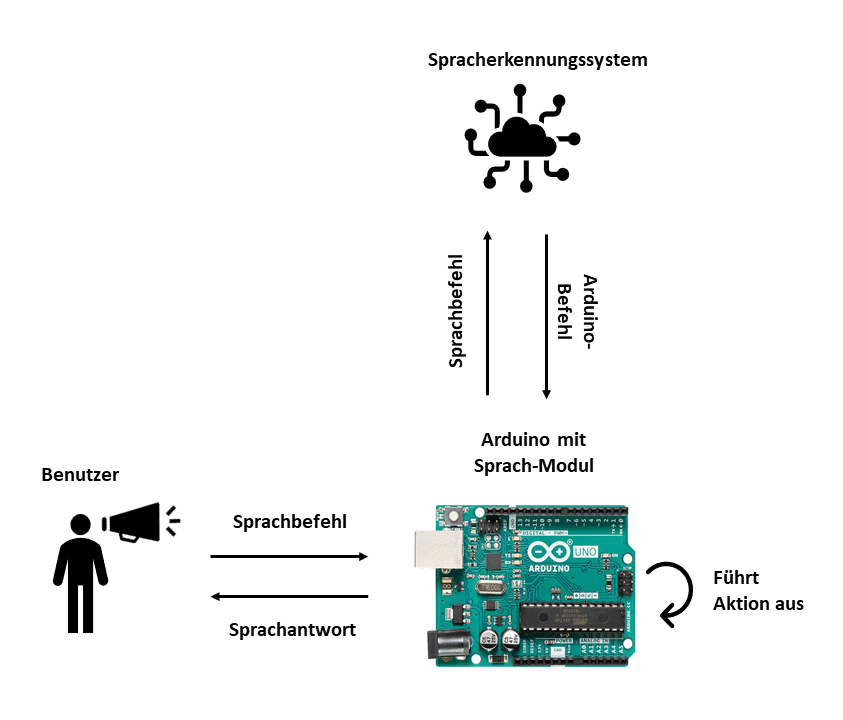
\includegraphics[width=0.9\textwidth]{Bilder_Kapitel_3/Konzept_A.jpg}}
    \caption{\label{figure:Spracherkennung_mittels_Arduino}Spracherkennung und -verarbeitung mittels Arduino}
\end{figure}
\section{Konzept B: Spracherkennung und -verarbeitung mittels mobiler Anwendung}
\section{Konzept C: Spracherkennung und -verarbeitung auf Computer-Hardware}
\section{Konzept D:}
\section{Finales Konzept}
\endinput




\chapter{Implementierung}
\section{Implementierung des Sprachverarbeitungssystems}
\subsection{Word2Vec-Modell}
\subsection{Sequence-to-Sequence-Modell}
\section{Befehlsverarbeitung in der Mischmaschine}
\section{Anbindung des Sprachmodells an die Mischmaschine}
\endinput



\chapter{Fazit und Ausblick}

TODO





% Ab hier beginnt der Anhang
\pagenumbering{roman}
\setcounter{page}{\value{roman-numbering}}
\appendix
% \addcontentsline{toc}{chapter}{Anhang}

% \addcontentsline{toc}{chapter}{Index}
\printindex

\addcontentsline{toc}{chapter}{Literaturverzeichnis}

% Haben Sie das "biblatex"-Paket nicht installiert, benutzen Sie folgendes:
% Ohne das "biblatex"-Paket (s. bericht.sty) produziert folgendes
% "deutsche" Zitate in Literaturverzeichnissen gemaß der Norm DIN 1505,
% Teil 2 vom Jan. 1984.
% Die Zitatmarken werden alphabetisch nach Verfassern
% sortiert und sind durch abgekürzte Verfasserbuchstaben plus
% Erscheinungsjahr in eckigen Klammern gekennzeichnet.

% \bibliographystyle{alphadin}
% \bibliography{bericht}

%%%%%%%%%%%%%%%%%%%%%%%%%%%%%%%%%%%%%%%5
% BIBLATEX
% Benutzt man das "biblatex"-Paket, muß man folgendes schreiben:
\def\refname{Literaturverzeichnis}
\printbibliography
%%%%%%%%%%%%%%%%%%%%%%%%%%%%%%%%%%%%%%%5


%%%%%%%%%%%%%%%%%%%%%%%%%%%%%%%%%%%%%%%%%%%%%%%%%%%%%%%%%%%%%%%%%%%%%%%%%%%%%%%%
%% Descr:       Vorlage für Berichte der DHBW-Karlsruhe, Änderungshistorie
%% Author:      Prof. Dr. Jürgen Vollmer, vollmer@dhbw-karlsruhe.de
%% $Id: changelog.tex,v 1.16 2020/03/13 15:12:39 vollmer Exp $
%% -*- coding: utf-8 -*-
%%%%%%%%%%%%%%%%%%%%%%%%%%%%%%%%%%%%%%%%%%%%%%%%%%%%%%%%%%%%%%%%%%%%%%%%%%%%%%%

\chapter*{Änderungen}

\begin{description}
\item[2020/03/13] Tippfehler korrigiert\\
                  aktuelle Formulierungen aus der Prüfungsordnung Technik übernommen\\
                  Formatdatei erklärt
\item[2017/10/06] Anpassung an neuer Versionen diverse Pakete.
\item[2016/03/16] Auf UTF-8 umgestellt, Indices.
\item[2010/04/12] ToDo-Markierungen mit dem \verb+\todo+-Kommando.
\item[2010/01/27] Anhang (\texttt{appendix}), Selbständigkeits-Erklärung, \texttt{framed}-Paket.
\item[2010/01/21] Abkürzungen (\texttt{acronym}), \texttt{table} und \texttt{tabular} benutzt,
     unübliche Pakete beigelegt.
\item[2010/01/18] Code-Listings (\texttt{listings}), Literaturreferenzen \texttt{biblatex})
\item[2010/01/11] Initiale Version.
\end{description}


\newpage
\addcontentsline{toc}{chapter}{Liste der ToDo's}
\listoftodos[Liste der ToDo's]


\end{document}
